\documentclass[12pt, twoside]{article}
\usepackage[francais]{babel}
\usepackage[T1]{fontenc}
\usepackage[latin1]{inputenc}
\usepackage[left=7mm, right=7mm, top=5mm, bottom=5mm]{geometry}
\usepackage{float}
\usepackage{graphicx}
\usepackage{array}
\usepackage{multirow}
\usepackage{amsmath,amssymb,mathrsfs}
\usepackage{soul}
\usepackage{textcomp}
\usepackage{eurosym}
 \usepackage{variations}
\usepackage{tabvar}


\pagestyle{empty}

\begin{document}


\begin{center}
\textbf{\Large{Devoir maison 6}}
\end{center}

\bigskip



\textit{Devoir � rendre sur feuille grand format pour le \ul{vendredi 28
mars 2014}. Chaque r�ponse devra �tre justifi�e.}

\bigskip


\bigskip

\ul{Exercice 1:} \textit{(2 points)}

\enskip


\begin{tabular}{cc}
\begin{minipage}{14cm}
Calculer la longueur KJ. On donnera une valeur arrondie au millim�tre pr�s.
\end{minipage}
&
\begin{minipage}{4cm}
\begin{center}
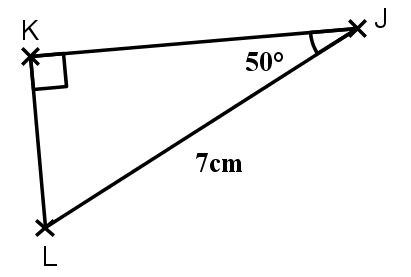
\includegraphics[width=4cm]{images/ex1.png}
\end{center}
\end{minipage}
\end{tabular}

\bigskip

\bigskip

\ul{Exercice 2:} \textit{(3 points)}


\begin{enumerate}
  
  \item GHI est un triangle rectangle en G tel que GH=6cm et
  $\widehat{GHI}$=30�. Construire cette figure en vraie grandeur.
  \item Calculer la longueur HI. On donnera une valeur arrondie au millim�tre
  pr�s.
\end{enumerate}



\bigskip

\bigskip

\ul{Exercice 3:} \textit{(5 points)}

\enskip

\begin{tabular}{cc}
\begin{minipage}{12cm}
\begin{enumerate}
  \item D�montrer que le triangle TIR est rectangle en I.
  \item Calculer la mesure de l'angle $\widehat{IRT}$. On donnera une valeur
  arrondie au dixi�me de degr� pr�s.
  \item En d�duire la mesure de l'angle $\widehat{ITR}$. Justifier votre
  r�ponse.
\end{enumerate}
\end{minipage}
&
\begin{minipage}{6cm}
\begin{center}
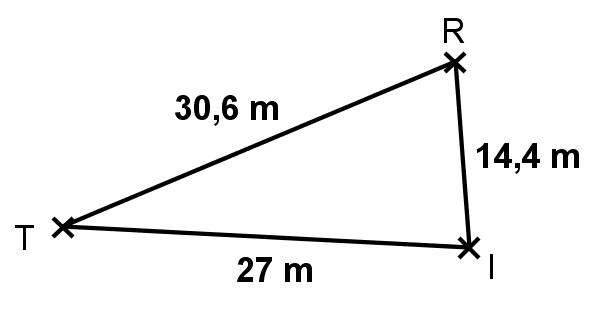
\includegraphics[width=5cm]{images/ex3.png}
\end{center}
\end{minipage}
\end{tabular}

\bigskip

\bigskip

\ul{Exercice 4:} \textit{(5 points)}

\enskip


Lors d'une sortie � la montagne avec les professeurs d'EPS, les �l�ves de
$4^{e}$ d'un coll�ge utilisent un t�l�ph�rique du Mont Toutenhaut  � la vall�e
Toutenbas. La distance horizontale entre le mont et la vall�e est de 852 m et
l'angle que fait le c�ble avec l'horizontale est de 25�. On admettra que le
c�ble est parfaitement rectiligne.

\enskip

\begin{tabular}{cc}
\begin{minipage}{10cm}
\begin{enumerate}
  \item Faire un sch�ma.
  \item Calculer la longueur du c�ble du t�l�ph�rique. On arrondira au m�tre la
  valeur trouv�e.
  \item Calculer de deux fa�ons (diff�rentes) la hauteur du mont au m�tre pr�s.
  
\end{enumerate}

\end{minipage}
&
\begin{minipage}{7cm}
\begin{center}
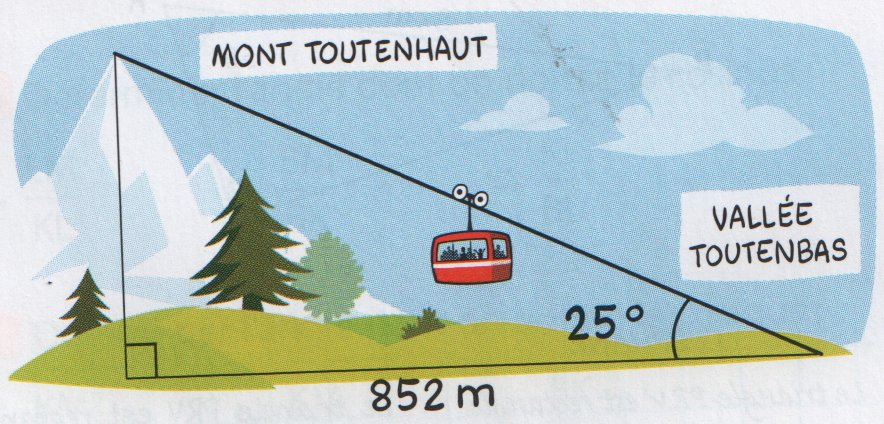
\includegraphics[width=7cm]{images/ex4.jpg}
\end{center}
\end{minipage}
\end{tabular}

\bigskip

\bigskip


\ul{Exercice 5:} \textit{(5 points)}

\enskip

\begin{tabular}{cc}
\begin{minipage}{13cm}
\begin{enumerate}
  \item Que peut-on dire des droites (BC) et (DE)? Justifier votre r�ponse.
  \item Calculer la longueur BC. Justifier votre r�ponse.
  \item Calculer la mesure de l'angle $\widehat{ACB}$. On donnera une valeur
  arrondie au degr� pr�s.
  \item En d�duire une mesure de l'angle $\widehat{AED}$. Justifier votre
  r�ponse.
\end{enumerate}
\end{minipage}
&
\begin{minipage}{5cm}
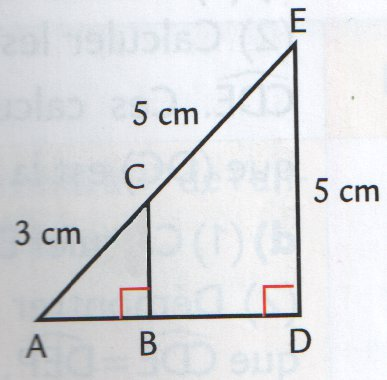
\includegraphics[width=4cm]{images/ex5.jpg}
\end{minipage}
\end{tabular}
\end{document}
